\documentclass[10pt,twocolumn]{article}

\usepackage{graphicx}
\usepackage{subfigure}
\usepackage{url}

\newcommand{\stufigex}[5]					% images with specified placement
{
	\begin{figure}[#5]
	\begin{center}
		\includegraphics[#1]{#2}
		\caption{#3}
		\label{#4}
	\end{center}
	\end{figure}
}

% Define the stusubfig environment
\newenvironment{stusubfig}[1]
{
	\begin{figure*}[#1]
	\begin{center}
}
{
	\end{center}
	\end{figure*}
}

\begin{document}

\title{Implementing Automatic Navigation Mesh Generation in Configuration Space}
\author{Stuart Golodetz}
\date{}
\maketitle

\section{Introduction}

The representation of the walkable area of a 3D environment in such a way as to facilitate successful navigation by intelligent agents is an important problem in the computer games and artificial intelligence fields, and it has been extensively studied. As surveyed by Tozour \cite{tozour04}, there are a variety of common ways to represent such an environment, including regular grids, which support random-access lookup but do not translate easily into a 3D context, use a lot of memory and can yield aesthetically unpleasing paths; waypoint graphs -- connecting large numbers of nodes (often manually placed) with edges that imply walkability in the game world -- these were previously popular in games but are costly to build and tend to constrain agents to walking `on rails' between connected waypoints; space-filling volumes, which entail growing randomly-placed seeds to try and fill the free space in the level; and navigation meshes, that represent the walkable surface of a world explicitly using a polygonal mesh. Polygons within a navigation mesh are connected using links that imply the ability of the agent to walk/step/jump/etc.\ between them (see Figure~\ref{fig:1}).

%---
\stufigex{width=.9\linewidth}{blakeney-midramp-neg.png}{An example navigation mesh, rendered as a negative image to highlight the mesh and links.}{fig:1}{t}
%---

Since their introduction by Greg Snook \cite{snook00}, navigation meshes have proved to be a particularly successful approach due to their ability to represent the free space available around paths through the world (this is extremely useful because it provides the pathfinder with the information it needs to successfully avoid local obstacles). As a result, they have seen widespread use in both games themselves, and popular games engines such as Source and Unreal, and many games authors have contributed to their theoretical development (most notably in the \emph{Game Programming Gems} and \emph{AI Game Programming Wisdom} book series). There has also been significant interest from researchers in academia (e.g.~see \cite{hale09,kallmann10,pettre05,vantoll11}).

%---
\begin{stusubfig}{!t}
	\subfigure[Finding the intersection of a half-ray through the nearest vertex of the AABB with the plane]
	{\hspace{6mm}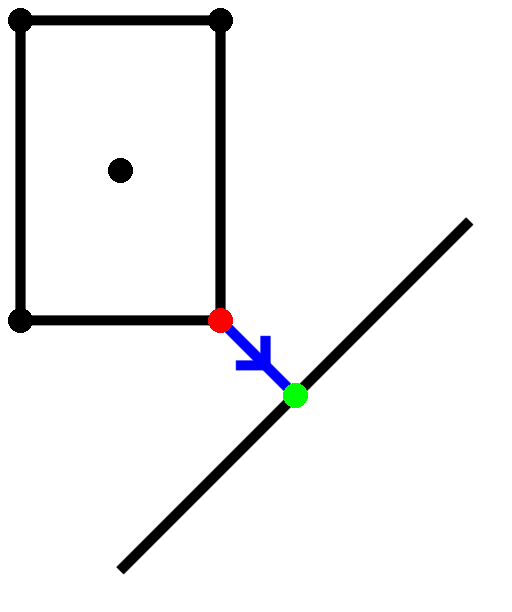
\includegraphics[width=.2\linewidth]{aabbvsplane-a.png}\hspace{6mm}}%
	%
	\hspace{10mm}%
	%
	\subfigure[Expanding the plane to form a configuration space]
	{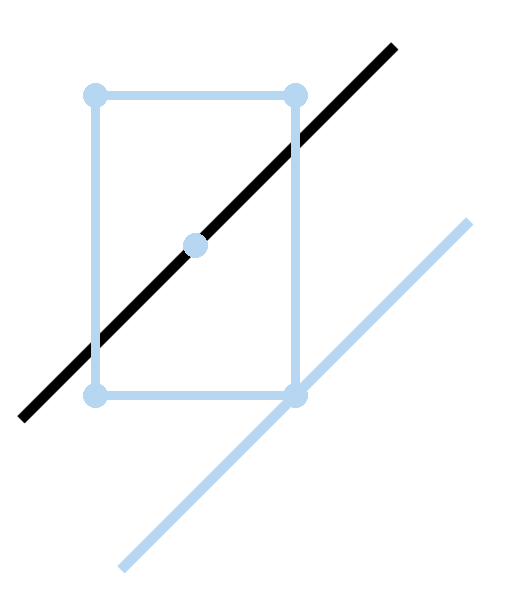
\includegraphics[width=.2\linewidth]{aabbvsplane-b.png}}%
	%
	\hspace{10mm}%
	%
	\subfigure[Finding the intersection of a half-ray through the centre of the AABB with the expanded plane]
	{\hspace{6mm}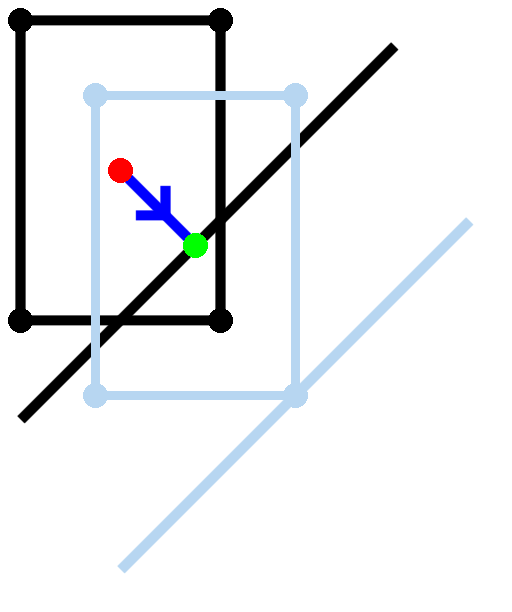
\includegraphics[width=.2\linewidth]{aabbvsplane-c.png}\hspace{6mm}}%
\caption{Detecting the first collision point between a translating AABB and a plane.}
\label{fig:aabbvsplane}
\end{stusubfig}
%---

One facet of using navigation meshes is how to build them in the first place, and numerous methods have been described in the literature, of which a few examples are described here. An early approach due to Tozour \cite{tozour02} works by first determining the walkable polygons in a 3D environment by comparing their normals with the up vector, and then iteratively merging together as many polygons as possible using the Hertel-Mehlhorn algorithm \cite{hertel83,orourke94} and a $3 \rightarrow 2$ merging technique. Hamm \cite{hamm08} generates a navigation mesh using an empirical method that involves sampling the environment to create a grid of points, identifying a subset of points both on the boundary of and within the environment, and connecting these points to form a mesh. Ratcliff \cite{ratcliff08} creates a navigation mesh by tessellating all walkable surfaces in the world, merging the results together to form suitable nodes and then computing links between neighbouring nodes. Van Toll \emph{et al.} \cite{vantoll11} build a navigation mesh for a multi-layer environment by constructing a mesh based on the medial axis for each layer and then connecting the medial axes by `opening' the connections between the layers. The same authors later demonstrated how such a mesh could be dynamically modified \cite{vantoll12}. Mononen's open-source Recast library \cite{mononen09} first voxelizes the 3D environment before running a watershed transform \cite{beucher90,gonzalez02} on the walkable voxels and creating a mesh from the resulting partition of the walkable surface.

%TODO: Survey the various methods \cite{axelrod08,farnstrom06,hale11,kallmann10,mcanlis08,mononen09,oliva11,pettre05,ratcliff08,vanwaveren01,wein05}.

In this article, I describe the implementation of navigation mesh construction in my homemade \emph{hesperus} engine \cite{hesperus}, based heavily on the approach of van Waveren in \cite{vanwaveren01}. The goal is to provide a helpful, implementation-focused introduction for those with no prior experience in the area. At a high-level, the method is as follows:
%
\begin{enumerate}
\item Given a 3D environment made up of brushes (simple convex polyhedra, each consisting of a set of polygonal faces), and a set of axis-aligned bounding boxes (AABBs) used to represent the possible sizes of the agents that will navigate the environment, expand the brushes by appropriate amounts (see \S\ref{sec:configspace}) to create a set of expanded brushes for each AABB.
\item Using constructive solid geometry (CSG) techniques, union the expanded brushes for each AABB together to form a combined brush. Filter the faces of each combined brush to find those that are \emph{walkable} (judged by comparing their face normals with the up vector). This gives us the polygons of a navigation mesh for each AABB, but without any links to indicate how agents should navigate between them. See \S\ref{sec:meshgen}.
\item Generate walk and step links between the polygons of each navigation mesh (see \S\ref{sec:walkstep}) -- these indicate, respectively, that an agent can walk from one polygon of the mesh to another, or step up/down from one polygon to another. These links can be used to generate a graph for the purposes of path planning.
\end{enumerate}
%
The following sections look at each of these steps in more detail.

\section{Configuration Spaces}
\label{sec:configspace}

When planning the movement of intelligent agents (e.g.~robots), a \emph{configuration space} is the space of possible configurations in which an agent can validly exist. As a first example of what this concept means and when it can be useful, consider detecting the first point of collision between a plane and an AABB that is moving by translation only -- this might normally involve determining which vertex of the AABB is nearest to the plane and finding the point at which a half-ray oriented in the AABB's direction of movement and starting at that vertex would intersect the plane (see Figure~\ref{fig:aabbvsplane}(a)). The configuration space alternative is to initially expand the plane in the direction of its normal by a fixed amount so that the centre of the AABB touches the expanded plane precisely when the nearest vertex of the AABB touches the non-expanded plane (see Figure~\ref{fig:aabbvsplane}(b)). The first point of intersection can then be calculated by finding the point at which a half-ray starting at the centre of the AABB would touch the expanded plane (see Figure~\ref{fig:aabbvsplane}(c)) -- there is no longer a need to first determine which vertex is nearest to the plane. Put another way: by expanding the plane, we have created the space of possible configurations for the centre of the AABB, and thereby restricted our testing to making sure that the AABB's centre is always in a valid location.

As explained in \cite{vanwaveren01}, the concept of configuration space can be extended to an entire 3D environment, allowing us to test an agent represented as an AABB against such an environment using only point-based (rather than AABB-based) intersection tests: this was the approach taken in the popular \emph{Quake III Arena} game. Starting with a \emph{brush-based} 3D environment (i.e.~one that is built up by combining instances of simple convex polyhedra such as cuboids, cylinders and cones -- a common approach in 3D world editors), a configuration space for agents with a specific AABB can be constructed by expanding each brush by an appropriate amount (see Figure~\ref{?}). Note that expanding each brush correctly can require the introduction of additional \emph{bevel} planes as described in \cite{vanwaveren01} (see Figure~\ref{?}).

\iffalse

\section{Onion BSPs}
\label{sec:onionbsp}

Having expanded the brushes as described above, it is possible to combine them into a brush that represents the entire environment using a constructive solid geometry (CSG) union operation (see Appendix~E of \cite{golodetz06}). The polygons of the combined brush so generated can then be used to build a binary space partitioning (BSP) tree of the environment (see Figure~\ref{?}) using a conventional BSP-building approach (see Appendix~D of \cite{golodetz06}). This BSP tree can be used to decide whether or not any given point in space is within a wall of the environment, which can be used for both discrete, point-based collision detection (`is this entity now in a wall as a result of its movement this frame?') and continuous collision detection (`does the line segment representing this entity's movement during this frame intersect a wall at any point?').

However, as noted above, the configuration space we created by expanding the brushes is for a specific AABB -- that is, it will only work for entities of a particular size and in a particular pose. To support entities of different sizes, or ones that can change pose (e.g.~by crouching), we need to create a different type of BSP tree that this article will call an \emph{onion} BSP (for reasons that will be explained).

TODO

\fi

\section{Basic Mesh Generation}
\label{sec:meshgen}

TODO

\section{Walk and Step Link Generation}
\label{sec:walkstep}

TODO: Edge plane table construction, intervals, etc.

\section{Potential Extensions}

\subsection{Crouch Links}

TODO

\subsection{Ladder Links}

TODO

\subsection{Jump Links}

TODO

\section{Conclusions}

In this article, I have illustrated how to generate navigation meshes at an implementation level using an approach based on the work of van Waveren in \cite{vanwaveren01}. Whilst there are many alternative techniques for navigation mesh construction, as described in the introduction, this configuration space approach is useful because it allows us to avoid the difficulties regarding clearance height that have to be dealt with by other approaches; it also means that each agent occupies a single point on the mesh, completely avoiding the problems caused by an agent straddling multiple mesh polygons.

Navigation mesh \emph{generation}, however, is only part of the picture -- in a future article, I hope to write more about using navigation meshes for localisation, movement and path planning.

\section{Acknowledgements}

TODO

%\nocite{*}

\bibliographystyle{plain}
\bibliography{navmesh}

\end{document}